\chapter{Fuentes Reguladas Serie}

 \hspace{10pt}  \textbf{Ejercicio 1}:   A partir del  circuito mostrado en la figura
\ref{fuentes1}, hallar: a) capacitor más adecuado, b)  diodos
necesarios y  c) tensión de ripple presente en la carga.

\begin{figure}[h]
	\centering
	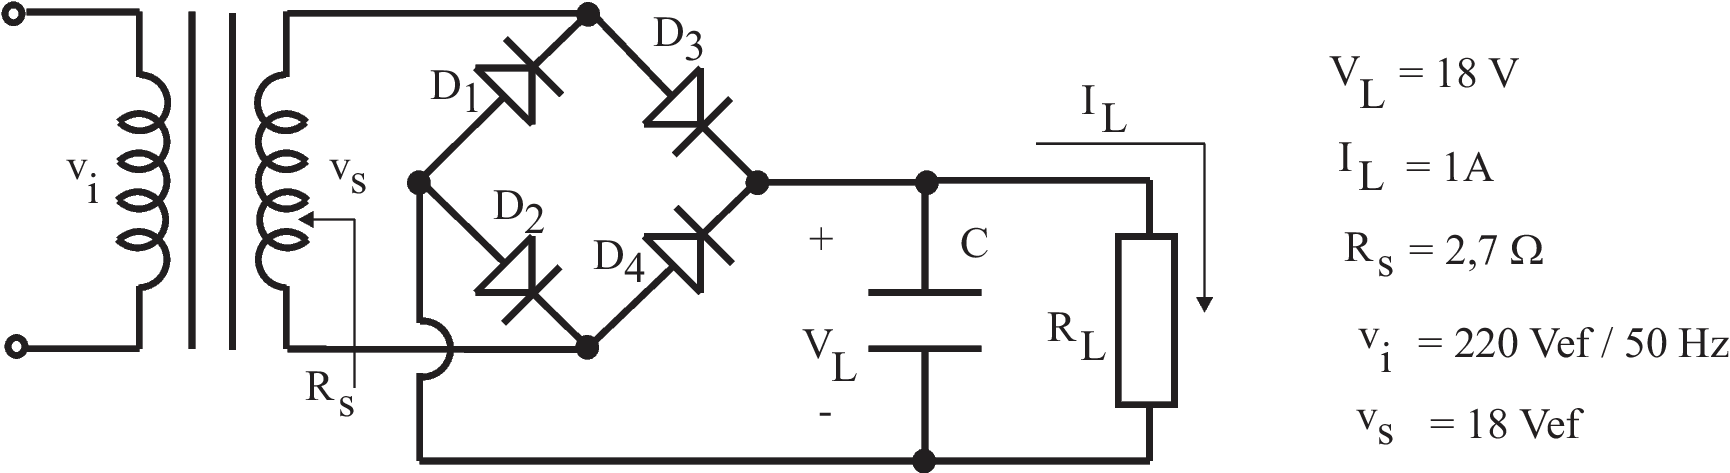
\includegraphics[width=0.6\linewidth]{figuras/fuentes1.png}\\
	\caption{Ejercicio 1.}\label{fuentes1}
\end{figure}

\textbf{Ejercicio 2} : En el  circuito de la figura \ref{fuentes2},
obtener: a) $R_x$,  b) $S_v = \frac{\displaystyle v_o}{\displaystyle
	v_f}$ y  c) $R_o$.

\begin{figure}[h]
	\centering
	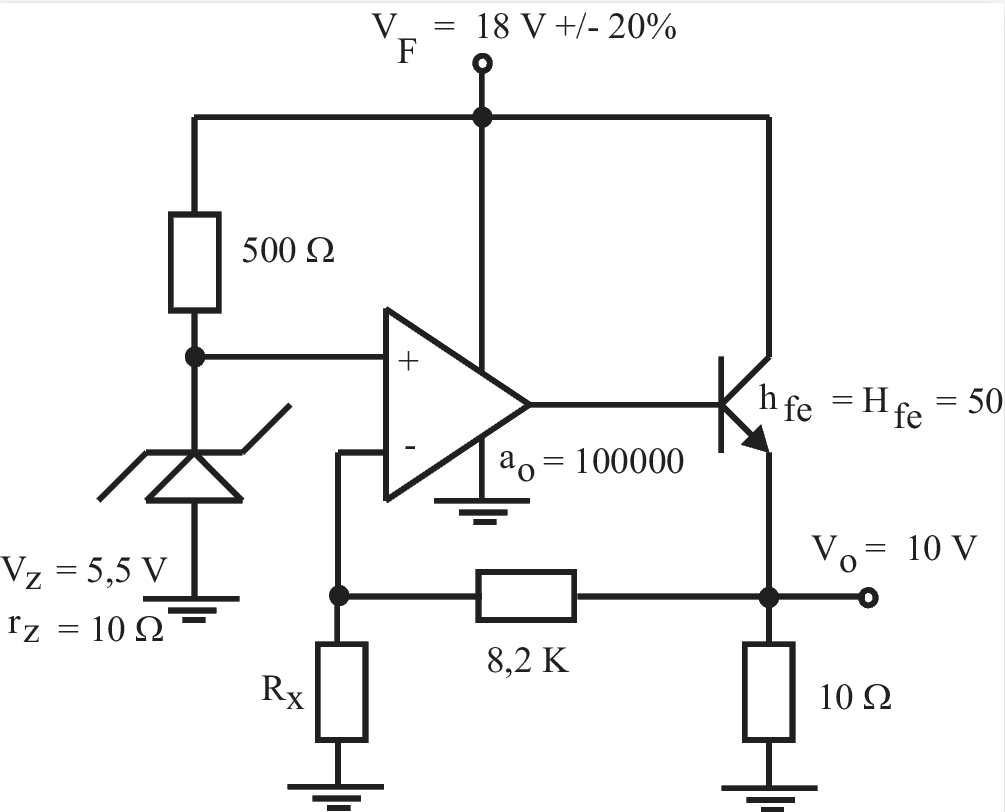
\includegraphics[width=0.5\linewidth]{figuras/fuentes2.png}\\
	\caption{Ejercicio 2.}\label{fuentes2}
\end{figure}

\textbf{Ejercicio 3}: En el circuito de la figura \ref{fuentes3}: a)
comparar con el diagrama en bloques básico de un regulador serie e
identificar cada bloque indicando los componentes que lo forman, b)
diseñar $R_1$ y $R_3$ de modo de obtener $V_0=8 V$ para $0 \leq  I_o
\leq 1 A$, c) calcular el factor de estabilidad $S_v$ y la
resistencia de salida $R_o$ y d) proponer una protección contra
cortocircuito en la salida.

\textbf{Ejercicio 4}: En el circuito de la figura \ref{fuentes4}
diseñar $R_x$, $R_A$ y $R_B$ para obtener una tensión regulada de
salida $V_o = 5V$ que pueda entregar una corriente de carga $0 \leq
I_L \leq 4 A $ suponiendo que el operacional tiene una ganancia $ a =
50000$, $R_0 \rightarrow 0$ y $R_i \rightarrow \infty $ y puede
entregar una corriente máxima $-3 mA \leq i_a \leq 3 mA$. Hallar el
factor de regulación de ripple $S_V$ y la resistencia de salida
$R_o$. Diseñar además una protección contra cortocircuito utilizando
el concepto de corriente de repliegue (fold back) asegurando que la
potencia disipada en $Q_1$ en condiciones de cortocircuito sea igual
a la máxima potencia disipada en $Q_1$ en funcionamiento normal.


\textbf{Ejercicio 5}: Diseñe una fuente regulada de tensión de 12 V
que pueda entregar hasta 1 A, utilizando las hojas de datos y notas
de aplicación adjuntas del circuito integrado $\mu A723$.


\begin{figure}[h]
	\centering
	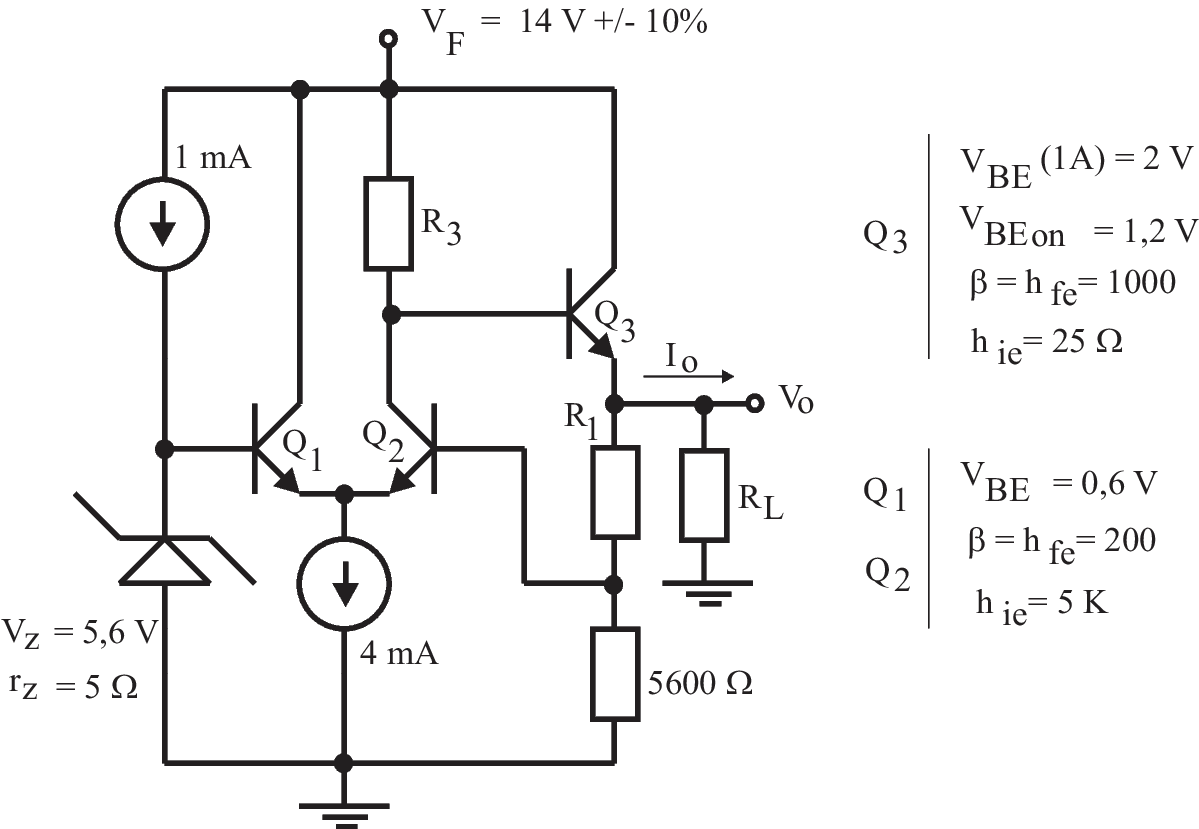
\includegraphics[width=0.6\linewidth]{figuras/fuentes3.png}\\
	\caption{Ejercicio 3.}\label{fuentes3}
\end{figure}

\begin{figure}[h]
	\centering
	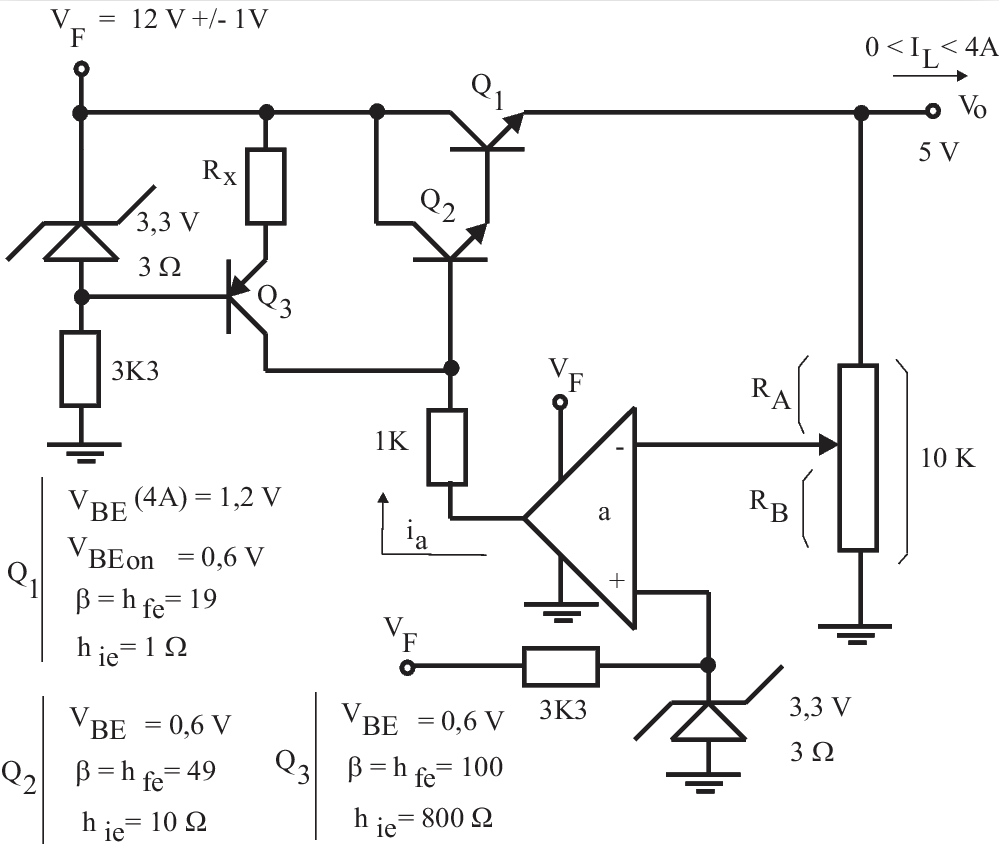
\includegraphics[width=0.6\linewidth]{figuras/fuentes4.png}\\
	\caption{Ejercicio 4.}\label{fuentes4}
\end{figure}

